%
% vergleich.tex
%
% (c) 2020 Prof Dr Andreas Müller, Hochschule Rapperswil
%
\begin{frame}
\frametitle{Vergleich}
\vspace{-15pt}
\begin{columns}[t]
\begin{column}{0.24\hsize}
\begin{block}{Euler vorwärts}
\vspace{-15pt}
\begin{align*}
Au_j
&=
u_{j+1} - u_j
\\
u_{j+1} &= (A+E)u_j
\end{align*}
\end{block}
\end{column}
\begin{column}{0.27\hsize}
\begin{block}{Euler rückwärts}
\vspace{-15pt}
\begin{align*}
Au_{j+1}
&=
u_{j+1} - u_j
\\
u_{j+1}
&=
(E-A)^{-1}
u_{j}
\end{align*}
\end{block}
\end{column}
\begin{column}{0.4\hsize}
\begin{block}{Crank-Nicholson}
\vspace{-15pt}
\begin{align*}
{\textstyle\frac12}(Au_j + Au_{j+1}) &= u_{j+1}-u_j
\\
({\textstyle\frac12}A-E)u_{j+1}&=-({\textstyle\frac12}A+E)u_j
\end{align*}
\end{block}
\end{column}
\end{columns}

\begin{columns}[t]
\begin{column}{0.24\hsize}
\begin{center}
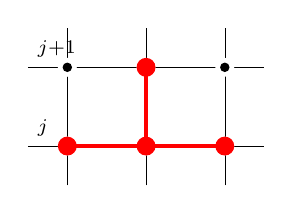
\begin{tikzpicture}[>=latex]
\draw[line width=0.2pt] (-1.5,0)--(1.5,0);
\draw[line width=0.2pt] (-1.5,1)--(1.5,1);
\draw[line width=0.2pt] (-1,-0.5)--(-1,1.5);
\draw[line width=0.2pt] (0,-0.5)--(0,1.5);
\draw[line width=0.2pt] (1,-0.5)--(1,1.5);
\foreach \x in {-1,...,1}{
	\foreach \y in {0,1}{
		\fill[color=white] (\x,\y) circle[radius=0.12];
		\fill (\x,\y) circle[radius=0.06];
	}
}
\fill[color=red] (-1,0) circle[radius=0.12];
\fill[color=red] (0,0) circle[radius=0.12];
\fill[color=red] (1,0) circle[radius=0.12];
\fill[color=red] (0,1) circle[radius=0.12];
\draw[color=red,line width=1.5pt] (-1,0)--(1,0);
\draw[color=red,line width=1.5pt] (0,0)--(0,1);
\node at (-1.5,1) [above right] {$\scriptstyle j+1$};
\node at (-1.5,0) [above right] {$\scriptstyle j$};
\end{tikzpicture}
\end{center}
\end{column}
\begin{column}{0.27\hsize}
\begin{center}
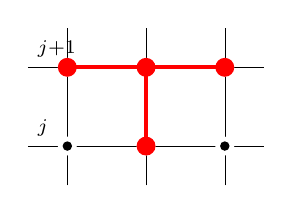
\begin{tikzpicture}[>=latex]
\draw[line width=0.2pt] (-1.5,0)--(1.5,0);
\draw[line width=0.2pt] (-1.5,1)--(1.5,1);
\draw[line width=0.2pt] (-1,-0.5)--(-1,1.5);
\draw[line width=0.2pt] (0,-0.5)--(0,1.5);
\draw[line width=0.2pt] (1,-0.5)--(1,1.5);
\foreach \x in {-1,...,1}{
	\foreach \y in {0,1}{
		\fill[color=white] (\x,\y) circle[radius=0.12];
		\fill (\x,\y) circle[radius=0.06];
	}
}
\fill[color=red] (-1,1) circle[radius=0.12];
\fill[color=red] (0,1) circle[radius=0.12];
\fill[color=red] (1,1) circle[radius=0.12];
\fill[color=red] (0,0) circle[radius=0.12];
\draw[color=red,line width=1.5pt] (-1,1)--(1,1);
\draw[color=red,line width=1.5pt] (0,0)--(0,1);
\node at (-1.5,1) [above right] {$\scriptstyle j+1$};
\node at (-1.5,0) [above right] {$\scriptstyle j$};
\end{tikzpicture}
\end{center}
\end{column}
\begin{column}{0.4\hsize}
\begin{center}
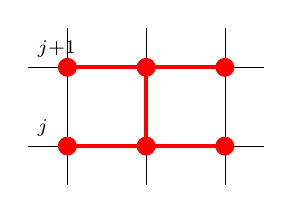
\begin{tikzpicture}[>=latex]
\draw[line width=0.2pt] (-1.5,0)--(1.5,0);
\draw[line width=0.2pt] (-1.5,1)--(1.5,1);
\draw[line width=0.2pt] (-1,-0.5)--(-1,1.5);
\draw[line width=0.2pt] (0,-0.5)--(0,1.5);
\draw[line width=0.2pt] (1,-0.5)--(1,1.5);
\foreach \x in {-1,...,1}{
	\foreach \y in {0,1}{
		\fill[color=red] (\x,\y) circle[radius=0.12];
	}
}
\draw[color=red,line width=1.5pt] (-1,1)--(1,1);
\draw[color=red,line width=1.5pt] (-1,0)--(1,0);
\draw[color=red,line width=1.5pt] (0,0)--(0,1);
\node at (-1.5,1) [above right] {$\scriptstyle j+1$};
\node at (-1.5,0) [above right] {$\scriptstyle j$};
\end{tikzpicture}
\end{center}
\end{column}
\end{columns}

\begin{columns}[t]
\begin{column}{0.24\hsize}
\begin{block}{Spektralradius\strut}
\vspace{-15pt}
\[
\varrho(A+E) = 38.990
\]
instabil
\end{block}
\end{column}
\begin{column}{0.27\hsize}
\begin{block}{$\Delta x = 0.1$\strut}
\vspace{-15pt}
\[
\varrho((E-A)^{-1}) = 0.99528
\]
stabil
\end{block}
\end{column}
\begin{column}{0.4\hsize}
\begin{block}{$\Delta t=0.1$\strut}
\vspace{-15pt}
\[
\varrho(
({\textstyle\frac12}A-E)^{-1}
({\textstyle\frac12}A+E)
)
=
1
\]
``stabil''
\end{block}
\end{column}
\end{columns}

\end{frame}
